% Any percent sign marks a comment to the end of the line
\documentclass[12pt,a4paper]{article}
\usepackage[utf8]{inputenc}
\usepackage{array}
\usepackage{amsmath}
\usepackage{amsfonts}
\usepackage{amssymb}
\usepackage{graphicx}
\usepackage{booktabs}
\usepackage{algorithm}
\usepackage{algpseudocode}
\usepackage{subcaption}
\usepackage[english]{babel}
\usepackage[export]{adjustbox}
\usepackage{enumerate}
\usepackage[left=3.5cm,right=2.5cm,top=2.5cm,bottom=2.5cm]{geometry}
\usepackage{lineno}
\usepackage{cite}
\usepackage{acronym}
\renewcommand{\baselinestretch}{1.5}



\begin{document}

	\begin{center}
		\begin{LARGE}			\bf{Paper Writeup\\}
		\end{LARGE}
		\vspace*{30pt}
		\textbf{Applied Digital Image Processing}
		\vspace{40pt}
		
		\textbf{
			Shayan Shoaib Patel (Student ID: sp07101)\\
			Muhammad Areeb Kazmi (Student ID: mk07202 )\\
            Group 12}\\

		\vspace{30pt}
		
\includegraphics[width=0.3\textwidth]{./logo.png} \\
		\vspace{30pt}
		\textit{Under the kind guidance of}\\
		\textbf{Dr. Muhammad Mobeen Movania}\\
		\textit{\textbf{Assistant Professor, Computer Science}}
		
		
		\vspace{20pt}
		
		
		\textbf{Dhanani School of Science And Engineering\\
			Habib University\\
			October 24, 2023
		}
	\end{center}

\pagenumbering{arabic}

% Every latex document starts with a documentclass declaration like this
% The option dvips allows for graphics, 12pt is the font size, and article
%   is the style

%\usepackage[pdftex]{graphicx}
%\usepackage{url}

% These are additional packages for "pdflatex", graphics, and to include
% hyperlinks inside a document.

\setlength{\oddsidemargin}{0.25in}
\setlength{\textwidth}{6.5in}
\setlength{\topmargin}{0in}
\setlength{\textheight}{8.5in}

% These force using more of the margins that is the default style


% Everything after this becomes content
% Replace the text between curly brackets with your own


% You can leave out "date" and it will be added automatically for today
% You can change the "\today" date to any text you like


% \maketitle

% This command causes the title to be created in the document
\newpage
\section{Introduction}
In the context of our present ecological challenges, addressing and raising awareness about global warming stands as a paramount imperative. Given the limitations in resources and the potential reluctance of governing bodies to prioritize this issue adequately, it becomes essential to pioneer a systematic approach for monitoring, reflecting upon, and mitigating these environmental changes.

Our primary objective is to institute a meticulous process for the collection and analysis of satellite imagery. Subsequently, we intend to apply various advanced methodologies and mathematical algorithms to these images. This multifaceted approach serves a dual purpose: it enhances our ability to comprehensively analyze and document alterations in land topography brought about by climate change, while also diminishing our reliance on local authorities and potential vested interests that may obstruct progress in this crucial area.

By implementing this approach, we aspire to foster greater transparency, accountability, and data-driven decision-making in the quest to combat global warming. Moreover, this initiative carries the potential to engage and enlighten the public about the pressing need for environmental conservation, ultimately leading to a more sustainable and resilient future for our planet.
% An article style is separated into sections and subsections with 
%   markup such as this.  Use \section*{Principles} for unnumbered sections.


\section{Motivation}
The motivation behind the proposal is to work with a real world problem which is significant to the survival of human species.
Deforestation is one of the by-products of the climate change that has contributed to the global warming. Keeping the context of
the course in mind, we aim to use techniques and knowledge acquired in the course to try to improve the process of identifying deforestation and the effects brought
by the anthropocene.
\newline The satellite technology accompanied with the high=resolution imagery can be a game changer in the monitoring and identification of deforestation and urban expansion.
\newline Our project aims to utilize the capabilities and functionalities of digital image processing to create a system for the purpose mentioned above that can be done using satellite imagery.
Here are some of the key motivations behind the project:
\subsection[2.1]{Environmental Impact}
Keeping in mind, the disastrous effects of industrialization and urbanization, the face of our planet has been changing in the modern times. Deforestation is a major contributor towards
the global boiling, as environmentalists term it now (instead of global warming). The monitoring system can contribute towards helping the relevant stakeholders to make better informed decisions through sustainable development.

\subsection[2.2]{Utilizing the true essence of Computer Science}
To our limited understanding, Computer Science has been the field of study that has been involved in solving problems that exist in the world. In fact, vast collaborations with practitioners, theorists, biologists, chemists, and people of other
professions have led to the innovation of new tools, applications, and opportunities. The same analogy can be directed towards solving a part of the problem of climate change and deforestation. By deploying suitable machine learning algorithms, image classification, and object detection methods, if possible,
we might be able to experience the very same essence of CS in this course.
\newline  
\newline Apart from the technical aspects, the project will also give us the opportunity to pitch ideas to relevant stakeholders, conduct the various phases of the project by managing it on time, and improve our own skillset and knowledge arsenal.
This project will help us to make a meaningful impact while gaining invaluable experience in the area of applied digital image processing.

\section{Literature Review}
We have identified a few papers that are relevant to our project. The papers from the year 2012 and onwards were handpicked to show the developments in both, classical and deep-learning and artificial intelligence based digital image processing. Most of the techniques use remote sensing, i.e., making use of the satellite imagery to detect image change and finally deforestation.

%Taken from Paper 3

\subsection[3.1]{Image Segmentation, Otsu Method}
Image Segmentation is seperating or dividing of images into different clusters or regions based on common properties and/or differences between other regons properties. One property out of the many could be applied to separating images into regions is pixel intensity. 

So we normally can segment images into different regions through thresholding or separating the pixel levels into different scales. These different thresholding scales create different regions corresponding to the pixel intensity values. 
\newline A simple example can be thresholding a gray scale image pixels into two regions, by transforming the gray scale image into binary image, which will consist of only two regions, namely either the black or white.

If $G(x,y)$ is a threshold version of $f(x,y)$ at some global threshold $T$,:
\[G(x,y) =
\begin{cases}
1 & \text{if } f(x,y) \geq T\\
0 \text{otherwise}
\end{cases}
\]

This is OTSU method named after Nobuyuki Otsu, which is a histogram shape-based method of image segmentation that sets thresholding value automatically. [Cite Otsu Method 1]

%Taken from Paper 3

\subsection[3.2]{Image Clustering} 
Content Based Image Clustering (CBIR) is a method used to group or classify objects into different classes which have similar properties. These classifying of images help us study different characteristics of 

This classifying of images into groups help assist study different characteristics of the image like better flow, pattern changes and similarity of events or phenomenon. Further clustering of images gives clusters or regions with detailed and concise information and the content of the images which ease the task of asserting this regions of clusters. FCM (Fuzzy C-mean) is one of the most common form of image clustering and it is the based on the principle of fuzzy classification. In fuzzy C-mean clustering pixels with identical properties will be grouped into to same categories or clusters. [Cite 2 Doc 22]

The input images of the fuzzy C-mean clustering, where Gray scale images and the cluster centers were computed automatically by the function itself. Once the cluster center was found and fixed, the next stage was setting the rules for fuzziification. That is if-then rules are given below assuming that the three cluster values are cluster 1, 2 and 3.
\begin{itemize}
	
	\item If pixel (i,j) is less than Cluster-1, center make it black(0)
		%\centering
	\item If pixel (i,j) is greater than cluster-3 center make it White (1).
		%\centering
	\item Else make pixel (i,j) in between black and white (0.5). 	
	%\end{flushleft}
\end{itemize}

The FCM algorithm continuously upgrades and moves this cluster centers iteratively to the ideal or right position. So by continuous moving of initial cluster centers, it precisely clusters the image into different regions and groups the accuracy of the membership grades of each groups [Cite3 in 23 in Doc]. 

% paper 2 used

\subsection[3.3]{Image ratioing}
Ratioing is considered to be relatively rapid means of identifying areas of change. In ratioing two registered images from different dates with one or more bands in an image are ratioed, band by band. The data are compared on a pixel or pixel basis. 

\begin{equation}
R(x) = \frac{I_{1}(x)}{I_{2}(x)}
\end{equation}

If the intensity of reflected energy is nearly the same in each image of R(x)=1, this indicates no change. In areas of change, the ratio value would be significantly greater than one or less than one, depending upon the nature of the change between the two dates. 

% Paper 2 used

\subsection[3.4]{Change Vector Analysis}
The change vector analysis involves two variables, the magnitude of variation and the angle of the change vector.
The change vector is obtained by subtracting the images represented in vector form.
The first step of the CVA method is to find (Normalized Difference Vegetation Index) NDVI and (Bare Soil Index) BI values of both the images.

$NDVI = (NIR - RED) / (NIR + RED)$
\newline $BI = ((SWIR + RED) - (NIR + BLUE)) / ((SWIR + RED) + (NIR + BLUE))$

where $NIR$, $RED$, $SWIR$ and $BLUE$ are the spectral reflectance measurements acquired in the near-infrared, red, short wave infrared and blue regions.
Change vector of each pixel includes two components NDVI and BI, which are the 2 axes in Cartesian coordinate system. The start point and finish point of the change vector are the locations of pixel in NDVI-BI space. The magnitude of vector represents the change intensity and the direction of vector represents the change dimension 
Further calculations not only allow us to furhter divide the values into two different groups which do not only allow to see the land and forestation/plantation affected. [Cite 4 paper 4]

\subsubsection[3.4.1]{Tasseled Cap Transformation Method}
The tasseled cap transformation parameters of ETM+ imagery were used to calculate the Brightness, Greenness 
and Wetness components of each image. The Tasseled cap transformation coefficients derived for Landsat 7 ETM+ 
data by the EROS Data Center (Huang et al. 2002) are given in Table 2. Brightness is a weighted sum of all bands, 
defined in the direction of the principal variation in soil reflectance. Greenness is a contrast between the near infrared and visible bands. It is strongly related to the amount of green vegetation in the scene. Wetness relates to 
canopy and soil moisture. The brightness, greenness and wetness indexes are obtained for both the images.

\begin{figure}[h]
	\centering
	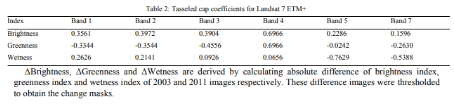
\includegraphics[width=0.7\linewidth]{./tasseledcap}
	% \caption{Tasseled Cap Transformation}
	\label{fig:tasseledcap}
\end{figure}

\subsubsection[3.4.2]{Principal Component Analysis Method}
The principal components transformation is a linear transformation which defines a new, orthogonal co-ordinate 
system such that the data can be represented without correlation. A bi-temporal feature space is constructed by 
placing the two image vectors in the same space. The transformation is found from the eigen vectors of the 
covariance matrix of the original data. Each individual pixel is transformed by vector multiplication of its original 
vector and the eigen vectors, resulting in coordinates in the new space. The transformed data is re-arranged back into
wo images corresponding to the first and second principal components. The first component images contain no change pixels whereas the second component images contain change information between the different dates.

Therefore, using the Brightness, Greenness and Wetness components of each image, the change vector analysis was performed. 

%Paper 9 used here

\subsection[3.5]{NDVI Method}
The approach is implemented using MATLAB. All band 
images were rotated 11 degrees with cubic interpolation. Then, 
the region of interest was cropped. Moreover, the missing lines in the satellite images are removed using 
the gray-level morphological closing operation. 
\newline Landsat 7 has eight bands: blue, green, red, near-infrared 1, 
near-infrared 2, thermal, mid-infrared, panchromatic. All of the 
bands have 30 meters resolution, except thermal with 60 and 
panchromatic with 15 meters of resolution (GIS Geography, 
2017, USGS, 2017)
\newline Picked bands of the imagery are band 2, 
band 3 and band 4, representing, green, red and near infrared 
bands. These bands are selected since they are used in the 
calculation of the NDVI. NDVI calculation is shown in equation below:
\begin{equation}
NDVI = \frac{NIR - RED}{NIR + RED}
\end{equation}
where $NIR$ and $RED$ are the near infrared and red bands respectively.
\newline Cropped images of these three bands are combined to form a 
false color composite image. 
Three other metrics are used, namely accuracy, precision, and recall.

Recall metric represents the rate of 
the correctly identified vegetated regions and calculated as TP / 
(TP + FN). On the other hand, precision indicates what 
percentage of the regions found as vegetation are actually true 
with respect to ground truth and calculated as TP / (TP + FP). 
Using precision and recall, we can calculate an fScore value for 
prediction of vegetated regions, which is a score varies in [0, 1] 
range. The higher the score value, the better the result is. The 
formula for fScore is shown in equation 3.

\begin{equation}
fScore = \frac{2 * Precision * Recall}{Precision + Recall}
\end{equation}

where Precision is the precision value for the case, Recall is the recall value for the case, and $fScore$ is the resultant $fScore$ that shows how good the result is.

Moreover, the vegetation ratio is also used to examine the loss in vegetation areas. Here, the total number of pixels with value 1 are divided by the total number of pixels.
\begin{equation}
Vegetation Ratio = \frac{Total Number of Pixels with Value 1}{Total Number of Pixels}
\end{equation}

%Paper 1 used here

\subsection[3.6]{Wavelength Method}
The data was processed and the analysis was by determining the wavelengths of certain frames from Landsat-7 and four frames from Landsat-8. The bands were combined for each frame and the null values were eliminated using the Copy Raster toolset. Finally, mosaicing was done on the frames for each year separately using the Mosaic to New Raster tool.
\newline The spatial-temporal variability
of normalized difference vegetation index NDVI was assessed to study deforestation using harmonic
analysis. We first spatially normalized observations to reduce seasonality. Subsequently, we detected
deforestation by assessing whether a newly acquired observation (satellite image) in the monitoring
period is in an extreme change when compared against spatially normalized values in present time data
defined over a reference period. The calculation of the NDVI for multi-date satellite images of Landsat
(7, 8) was used to perform change detection of the deforestation in Huambo Miombo.
\newline The
NDVI, as one of the most successfully used vegetation spectral indices, allows comparison between
inter-annual and seasonal changes in vegetation. The NDVI measures the amount of green vegetation
in an area and is used to distinguish forested from deforested areas.

\begin{figure}[h]
	\centering
	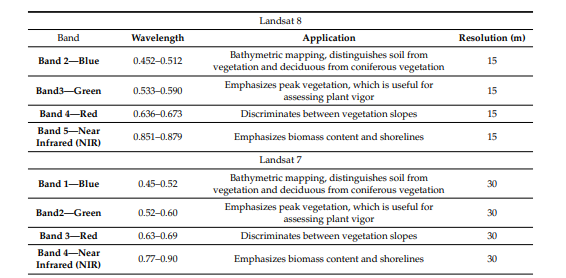
\includegraphics[width=0.7\linewidth]{./wavelength-9.png}
	\caption{Landsat Satellite Sensor characteristics}
	\label{fig:wavelength}
\end{figure}

\section{Methodology}

\section{Results}

\section{Conclusion}

\begin{thebibliography}{99}

\bibitem{minu} S. Minu, 
Amba Shetty,
{A Comparative Study of Image Change Detection Algorithms in MATLAB},
Aquatic Proc, {\bf 4}, 1366-1373 (2015), https://doi.org/10.1016/j.aqpro.2015.02.177.
% @article{minu,
%     author = "S. Minu, Amba Shetty",
%     title = "A Comparative Study of Image Change Detection Algorithms in MATLAB",
%     journal = "Aquatic Procedia",
%     volume = "4",
%     pages = "1366-1373",
%     year = "2015",
%     DOI = "https://doi.org/10.1016/j.aqpro.2015.02.177.",
%     keywords = "Change detection, Algorithms, Remote sensing, ETM+, Matlab, GUI"
%     }
\end{thebibliography}



\end{document}